% !Mode:: "TeX:UTF-8"
\chapter{系统详细设计与实现}

上一章从宏观上介绍了本系统的设计,这一章从微观出发,着重介绍中心路径提取模块的设计与实现。

在\ref{afmm-3D}节中讨论了3D中心路径提取算法的原理,这里,我们来看具体实现。
\section{数据结构说明}

DARRAY是一个动态数组,它可以在需要的时候动态扩展,并且它支持数据随机删除,类STACK继承自DARRAY。这个数据结构在实现里面保存点的时候很有用,图\ref{darray_class}是类图:
\begin{figure}[h!]
    \centering
    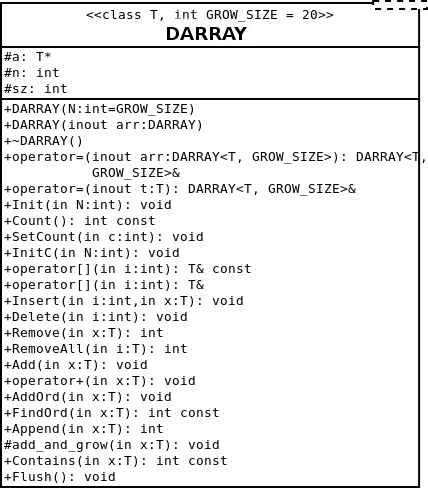
\includegraphics[width=300bp]{figure/darray.png}
    \caption{DARRAY类图}
    \label{darray_class}
\end{figure}

FIELD是一个模板类,它在逻辑上是一个二维矩阵。里面可以储存各种类型的变量。这个类是很关键的一个类,增强快速行进法处理的二维数据都是这个类的实例。
\begin{figure}[h1]
    \centering
    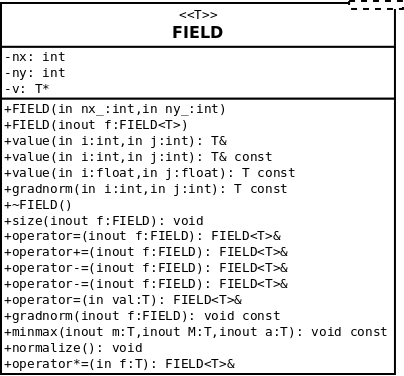
\includegraphics[width=300bp]{figure/field.png}
    \caption{FIELD类图}
    \label{field_class}
\end{figure}

前面有讲到,快速行进法中使用了一个标志$f_{ij}$(参看第\ref{pseudocode}节)。这个标志的实现是一个FLAGS类,它继承自FILED<int>。FLAGS有可能的值有几种,如代码\ref{flag-type}所示:
其中NARROW\_BAND表示BAND类型的点,它的值依然在演化中,也就是窄带上的点。ALIVE是KNOWN类型的点,它的值已经确定,即窄带后面已知点集($A^n$)里面的点。FAR\_AWAY就是INSIDE点,它的值目前还是未知的,即未知区域里面的点。还有一个EXTREMUM,这是一种特殊的已知点,他不仅是已知点,还是极值点。
\begin{lstlisting}[
    language={C},
    caption={FLAGS的类型},
    label={flag-type},
]
enum FLAG_TYPE {
    NARROW_BAND,
    ALIVE,
    FAR_AWAY,
    EXTREMUM
}
\end{lstlisting}

FLAGS的类图如图\ref{flags-class}所示。
\begin{figure}[h!]
    \centering
    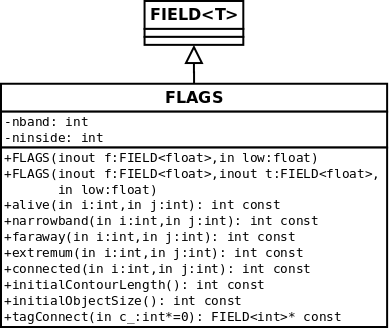
\includegraphics[width=300bp]{figure/flags.png}
    \caption{FLAGS类图}
    \label{flags-class}
\end{figure}

此外还有一个很重要的类就是VOLUME类,这个类在逻辑上是一个立方阵,存储3D物体的体数据。它可以读取体数据文件,生成实例,并且修改,保存体数据。由于体数据可以分割成一片一片,它还支持体数据的切片,拼接等功能。
VOLUME的类图如图\ref{volume-class}所示:
\begin{figure}[h!]
    \centering
    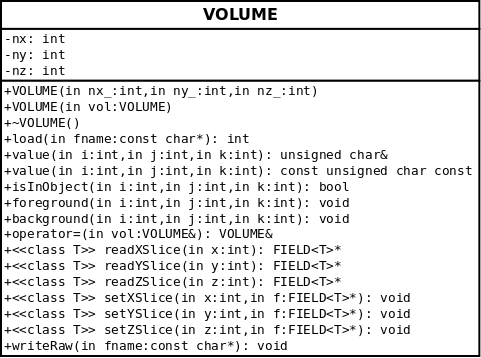
\includegraphics[width=300bp]{figure/volume.png}
    \caption{VOLUME类图}
    \label{volume-class}
\end{figure}

最后就是用于提取3D中心路径的skeleton类,这个类,提供了
